%%%%%%%%%%%%%%%%%%%%%%%%%%%%%%%%%%%%%%%%%%%%%%%%%%%%%%%%%%%%%%%%%%%%%%%%%%%%%%%%
\chapter{Разработка}
%%%%%%%%%%%%%%%%%%%%%%%%%%%%%%%%%%%%%%%%%%%%%%%%%%%%%%%%%%%%%%%%%%%%%%%%%%%%%%%%

Креатив.

%%%%%%%%%%%%%%%%%%%
\section{* Подходы к проблеме}
%%%%%%%%%%%%%%%%%%%

***

%%%%%%%%%
\subsection{Нисходящий однопроходный метод}
%%%%%%%%%

Основная идея -- спуск по дереву разбора (CST) от корневого узла к листьям, собирая по пути следования информацию для определения контекста, в котором находятся обрабатываемые/инструментируемые узлы.
\nomenclature{CST}{Concrete Syntax Tree -- конкретное дерево разбора}

Обход "в глубину" (DFT).
\nomenclature{DFT}{Deep-First Traversal -- метод обхода графовой структуры, при котором сначала будут обработаны все дочерние узлы текущего, ???}

***

Основная идея нисходящего подхода заключается в постепенном спуске по дереву разбора, которое генерирует внутри себя утилита TXL, от корневого узла к листьям, сохраняя по пути следования информацию для определения контекста, в котором находятся обрабатываемые узлы и выполняется инструментирование.

%%%%%%%%%
\subsection{Ограничения выбранного метода инструментирования}
%%%%%%%%%

***
Синтаксическое дерево исходного текста программы не содержит циклов по типам узлов -- при спуске от корня к листьям каждый тип узла встречается не более одного раза

%%%%%%%%%%%%%%%%%%%%%%%%%%%%%%%%%%%%%%%%%%%%%%%%%%%%%%%%%%%%%%%%%%%%%%%%%%%%%%%%
\section{Принцип работы системы}
%%%%%%%%%%%%%%%%%%%%%%%%%%%%%%%%%%%%%%%%%%%%%%%%%%%%%%%%%%%%%%%%%%%%%%%%%%%%%%%%

***
Ключевыми идеями системы являются:
\begin{itemize}
  \item Оперирование контекстами инструментирования как некоторыми множествами.
  \item Использование одного прохода по дереву разбора для осуществления требуемых манипуляций (вставки фрагментов программного кода).
\end{itemize}

%%%%%%%%%%%%%%%%%%%
\subsection{Взаимодействие с окружением}
%%%%%%%%%%%%%%%%%%%

***
как будет работать система?

На рис. ~\ref{fig:layout_artefacts} приведена обобщенная схема работы системы инструментирования с позиции манипуляции артефактами, такими как файлы и аргументы командной строки (параметры запуска).

\begin{figure}[!h]
	\centering
	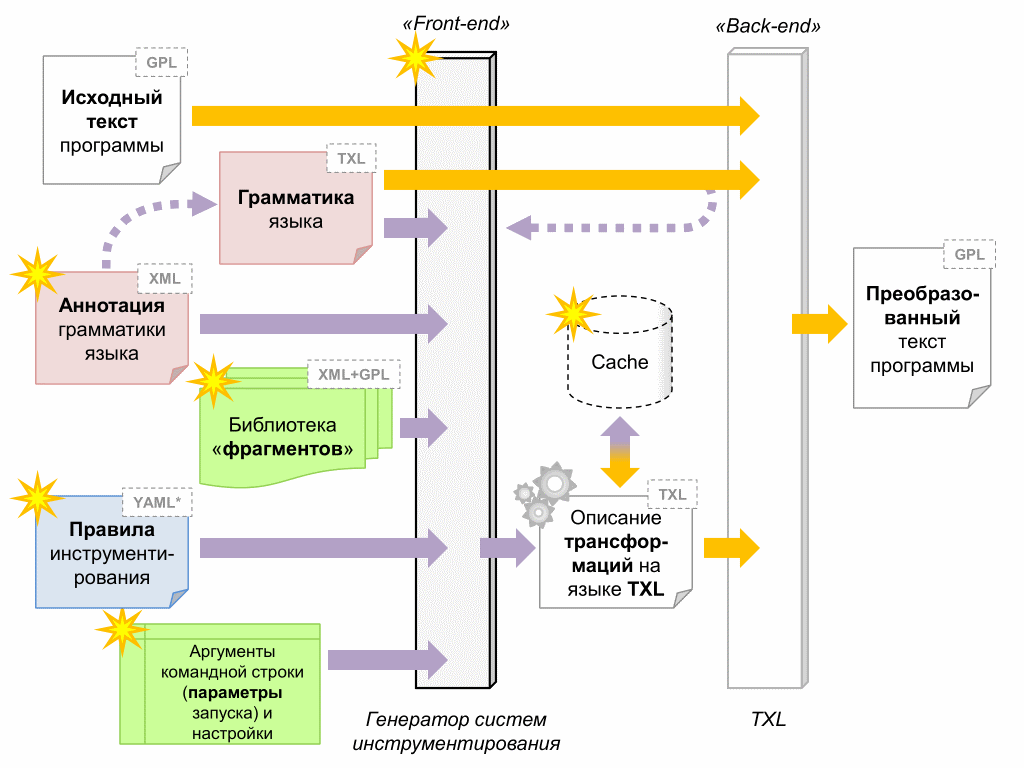
\includegraphics[width=4.2in]{layout_artefacts}
	\caption{Cхема работы системы. Артефакты.}
	\label{fig:layout_artefacts}
\end{figure}

для её работы необходимы:
\begin{itemize}
  \item Текст программы, инструментирование которой необходимо выполнить.
  \item Описание грамматики языка, на котором написан исходный текст этой программы.
  \item Аннотация грамматики языка.
  \item Пользовательские правила инструментирования.
  \item Фрагменты исходных текстов на выбранном языке программирования, вставку которых необбходимо выполнить.
  \item Дополнительные необязательные параметры запуска системы и переменные среды исполнения.
\end{itemize}

***

%%%%%%%%%%%%%%%%%%%
\subsection{Правила инструментирования}
%%%%%%%%%%%%%%%%%%%

***
про язык

На рис.~\ref{fig:layout_ruleset} приведен пример описания правил инструментирования с точки зрения конечного пользователя системы.

\begin{figure}[!h]
	\centering
	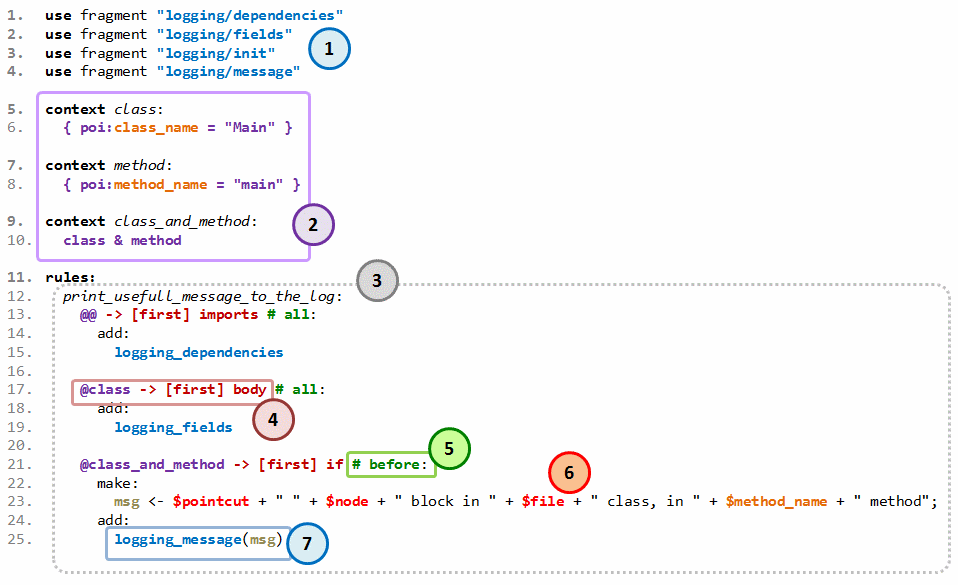
\includegraphics[width=4.2in]{layout_ruleset}
	\caption{Пример описания правил инструментирования}
	\label{fig:layout_ruleset}
\end{figure}

*описание частей*
\begin{enumerate}
  \item 11
  \item 22
  \item 33
  \item 44
  \item 55
  \item 66
  \item 77
\end{enumerate}

%%%%%%%%%%%%%%%%%%%
\subsection{Аннотация грамматики языка}
%%%%%%%%%%%%%%%%%%%

***
про XML

* Было бы удобно видеть в одном месте упрощенную схему иерархии типов узлов дерева разбора, в которой отображены только наиболее важные понятия, такие как "класс", "метод", "оператор ветвления", "цикл со счетчиком" и др.

%%%%%%%%%%%%%%%%%%%
\subsection{Фрагменты программного кода}
%%%%%%%%%%%%%%%%%%%

***
про XML

%%%%%%%%%%%%%%%%%%%
\subsection{Пользователи системы}
%%%%%%%%%%%%%%%%%%%

На рис. ~\ref{fig:layout_users} приведена схема работы системы инструментирования с позиции взаимодействия пользователей и системы как части производственного процесса (создания и отладки программного продукта).

\begin{figure}[h]
	\centering
	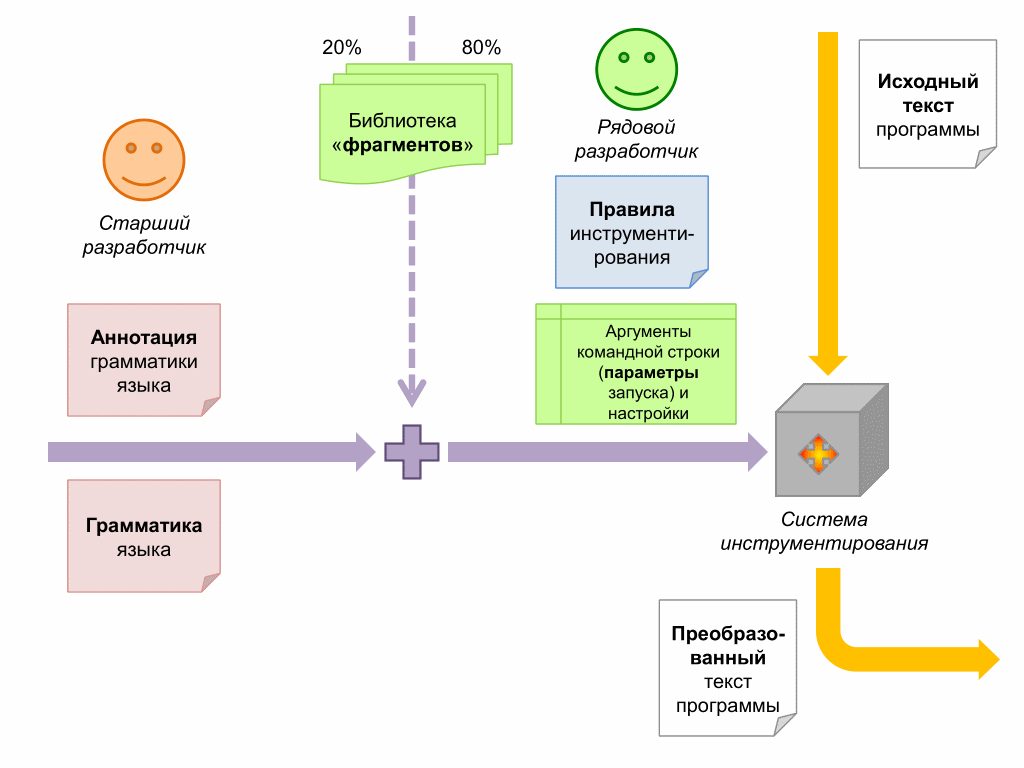
\includegraphics[width=4.2in]{layout_users}
	\caption{Cхема работы системы. Пользователи.}
	\label{fig:layout_users}
\end{figure}

***
с точки зрения пользователей есть два пользователя:

\begin{itemize}
  \item более опытный пользователь, в лице старшего разработчика в задачи которого входит:
    \begin{itemize}
      \item описание грамматики целевого языка программирования;
      \item составление аннотации к грамматике;
      \item отладка аннотации и грамматики;
      \item составление примеров фрагментов на целевом языке программирования.
    \end{itemize}

  \item конечный пользователь, в лице рядового разработчика в задачи которого входит:
    \begin{itemize}
      \item составление правил инструментирования;
      \item создание и пополнение библиотеки фрагментов исходных текстов на целевом языке;
      \item применение системы инструментирования к исходным текстам какой-либо программной системы.
    \end{itemize}
\end{itemize}

Исходя из задач, решаемых разными пользователями системы, можно выделить следующий минимальный набор компетенций для разных групп пользователей системы:
\begin{itemize}
  \item 111
  \item 222
\end{itemize}


%%%%%%%%%%%%%%%%%%%
\subsection{Выходные артефакты генератора}
%%%%%%%%%%%%%%%%%%%

***
про кэш

%%%%%%%%%%%%%%%%%%%%%%%%%%%%%%%%%%%%%%%%%%%%%%%%%%%%%%%%%%%%%%%%%%%%%%%%%%%%%%%%
\section{Выводы}
%%%%%%%%%%%%%%%%%%%%%%%%%%%%%%%%%%%%%%%%%%%%%%%%%%%%%%%%%%%%%%%%%%%%%%%%%%%%%%%%

Текст.
